\documentclass[12pt]{article}
\usepackage[utf8]{inputenc}
\usepackage[spanish, es-tabla]{babel}
\usepackage{graphicx}
\usepackage{float}


\title{Segmentación 3D de manchas de sustancia blanca (WML)}
\date{19/05/2019}
\author{J. Gamazo, G. Izaguirre, G. Cabrera \\
	 Universidad Nacional de Educación a Distancia}


\begin{document}
	\pagenumbering{gobble}
	\maketitle
	\newpage
	\paragraph{}
	\newpage
	\pagenumbering{arabic}
	\tableofcontents
	\newpage
	
	\renewcommand{\abstractname}{Resumen}

	\begin{abstract}
	En los últimos años, la visión artificial ha evolucionado enormemente, en parte gracias a métodos basados en deep learning. Esta evolución se ha aprovechado en medicina, puesto que se han creado métodos capaces de detectar distintas lesiones en imágenes como magneto-resonancias o radiografías, de forma automática. Fruto de ello, se han creado también diversos concursos para encontrar el mejor método en multitud de disciplinas distintas, estando uno de ellos centrado en la segmentación de manchas de sustancia blanca en el cerebro, lo cual podría ayudar a prevenir enfermedades vasculares entre otras. En este trabajo, se pretende mejorar los resultados obtenidos por uno de los métodos presentados a dicho concurso, por medio de técnicas de aumento de datos.
	\end{abstract}
	
	
	\renewcommand{\abstractname}{\textit{Abstract}}
	
	\begin{abstract}
	In the last years, artificial vision has evolved a lot, partly thanks to deep learning based methods. This evolution has benefited medicine, because there exist methods capable of detect several injuries by looking in images, such as MRI or X-ray, automatically. Besides, contests have been created to find the best method in different disciplines, being one of them focused on the segmentation of white matter hyperintensities, which could help to prevent vascular ills among others. In this work, the objective is to improve the results of one of the methods presented to that contests, using techniques of data augmentation.
	\end{abstract}

	\newpage
	
	\section{Introducción}

	\paragraph{}
	En 2017, en las conferencias MICCAI (\textit{Medical Image Computing and Computer Assisted Intervention}), fue lanzado el concurso de Segmentación de Hiperintensidades de materia blanca. Este se trata de un concurso de análisis de imágenes médicas, en el que se pretende comparar directamente métodos para la segmentación automática de Hiperintensidades de Materia Blanca en el cerebro.

	\paragraph{}
	El interés en este campo radica en que estas hiperintensidades se encuentran comúnmente en personas mayores y están asociadas con varios desórdenes neurológicos y geriátricos, como problemas de humor o deterioro cognitivo.

	\paragraph{}
	Normalmente son encontradas en magneto-resonancias FLAIR y, aunque es posible marcar las zonas donde se encuentran las hiperintensidades a mano, es una tarea bastante laboriosa. Es por ello que técnicas basadas en la visión artificial y en aprendizaje máquina han ganado mucho peso en los últimos año, como una forma bastante prometedora para el diagnóstico automático de enfermedades.

	\paragraph{}
	En cuanto al concurso, desde la propia organización se proporciona un conjunto de entrenamiento que todos los participantes deben descargar y usarlo para desarrollar su propio método, el cual debe ser contenedorizado con Dockers. El conjunto de test es guardado por la organización y no es hecho público en ningún momento, siendo únicamente utilizado para evaluar los distintos métodos. Para esta evaluación, además,  se han utlizado cinco métricas: coeficiente de similaridad de Dice, distancia de Hausdorff, diferencia absoluta de volumen, sensitividad para lesiones individuales y puntuación F1 para lesiones individuales.
	
	\paragraph{}
	En este artículo se presentan los cambios realizados en uno de estos modelos, en concreto el ganador, el cual hace uso de una variante de redes totalmente convolucionales basada en U-Net. Estos cambios han sido la creación de una GAN para conseguir un aumento significativo en el volumen de datos de entrenamiento. La razón de esta decisión es que los datos disponibles para el desarrollo de métodos no supervisados como el que se está llevando a cabo, son escasos y complicados de conseguir, puesto que expertos tienen que anotar manualmente cada una de las imágenes, siendo una tarea larga y tediosa. Por tanto, resulta conveniente aprovechar la capacidad de modelos generativos como las GAN para crear nuevas imágenes para usar durante el desarrollo de este modelo.
	
	\subsection{Estado del arte}

	\paragraph{}
	El método base a utilizar, descrito más en detalle en el artículo de Hongwei Li et al. \cite{Fully convolutional network ensembles for white matter hyperintensities segmentation in MR images}, ha sido el ganador de este concurso, y se basa en el uso de una variante de redes convolucionales basada en U-Net.
	
	\paragraph{}
	Así, su arquitectura toma como entrada los cortes axiales de dos modalidades de escáneres de magneto-resonancia, T1 y FLAIR, las cuales son juntadas como entrada de dos canales. En la imagen inferior se puede observar dicha arquitectura.
	
	\paragraph{}
	
	\begin{figure}[h!]
	\centering
		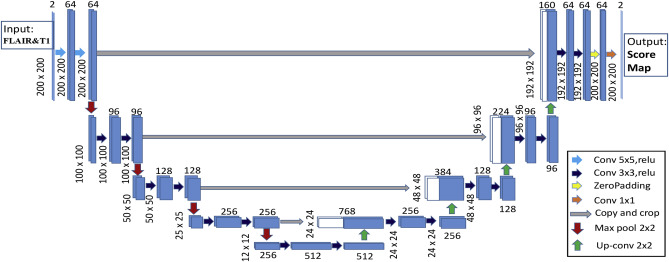
\includegraphics[width=\linewidth]{img1.jpg}
		\caption[\textit{Arquitectura del modelo}]{Arquitectura del modelo}
		\label{fig:FCC}
	\end{figure}

	\paragraph{}
	En este modelo, dos capas convolucionales son usadas de forma repetida, cada una seguida por una unidad de rectificado lineal (ReLU) y una operación max-pooling de 2 x 2 con paso 2. En la capa final, una convolución de 1 x 1 es utilizada para mapear cada vector de características de 64 componentes en dos clases. En total, se utilizan 19 capas convolucionales. 
	
	\paragraph{}
	Como función de pérdida se utiliza la pérdida de Dice, la cual es formulada de la siguiente forma:
	
	\begin{figure}[H]
	 	\centering
		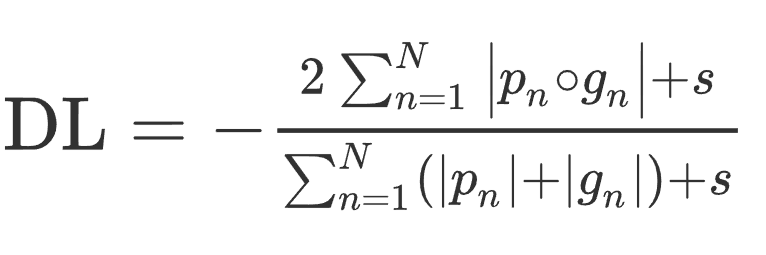
\includegraphics[height=2cm]{dice_loss.png}
		\label{fig:Dice}
	\end{figure}
	
	\paragraph{}
	donde G=\{g$_{1}$, .... g$_{N}$\} es la probabilidad observable de segmentación sobre N capas, y P=\{p$_{1}$, ..., p$_{N}'$\} la probabilidad predicha sobre N capas.
	
	\paragraph{}
	Por último, cabe mencionar que este método, como su nombre indica, utiliza técnicas de conjuntos, las cuales son útiles para reducir los problemas de exceso asociados a las redes neuronales. Estas combinan múltiples modelos de aprendizaje para obtener mejor rendimiento a la hora de predecir.
	
	\newpage
	
	\section{GAN: Generative Adversial Networks}
	
	\paragraph{}
	Para la realización de este proyecto, se ha decidido a utilizar redes GAN para conseguir un aumento de datos considerables, y que así el modelo descrito anteriormente pueda obtener mejores resultados. Por tanto, resulta conveniente en un primer momento, explicar el concepto de estas redes.
	
	\paragraph{}
	Las GAN, del inglés \textit{Generative Adversial Networks}, traducido al español como Red Generativa Antagónica, son un framework para estimar modelos generativos. Consisten en dos submodelos claramente diferenciables, típicamente implementados como redes neuronales: El generador \textit{G} y el discriminador \textit{D}. 
	
	\paragraph{}
	El funcionamiento de estas redes es sencillo. Por un lado, el generador es entrenado para generar imágenes \textit{G(z)} las cuales se parezcan a la distribución de los datos de entrenamiento \textit{p$_{R}$}, utilizando un vector de ruido latente \textit{z}, muestreado a partir de la distribución \textit{p$_{z}$}; mientras que el discriminador recibe tanto imágenes generadas como el conjunto de datos de entrenamiento real \textit{x}, y es entrenado para diferenciarlas.
	
	\paragraph{}
	De este modo, el generador es entrenado para minimizar la posibilidad de que el discriminador rechaze las imágenes generadas \textit{(D(G(z)) $\supset$ 0)}, mientras que el discriminador es entrenado para maximizar la probabilidad de acertar \textit{(D(G(z)) $\supset$ 0), (D(x) $\supset$ 1)}. Esto lleva a la siguiente función minimax:
	
	\begin{figure}[H]
	 	\centering
		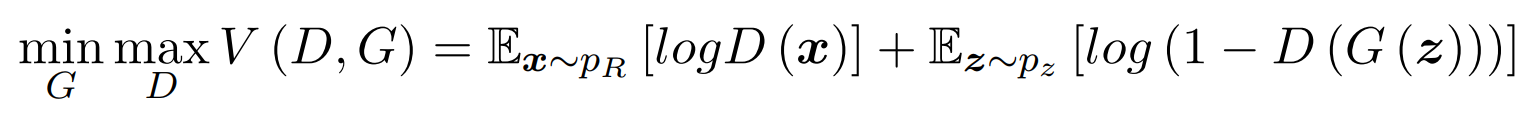
\includegraphics[height=1cm]{minimax.png}
		\label{fig:minimax}
	\end{figure}
	
	\paragraph{}
	A continuación se muestra un ejemplo de la arquitectura típica de una GAN:
	
	\begin{figure}[H]
	 	\centering
		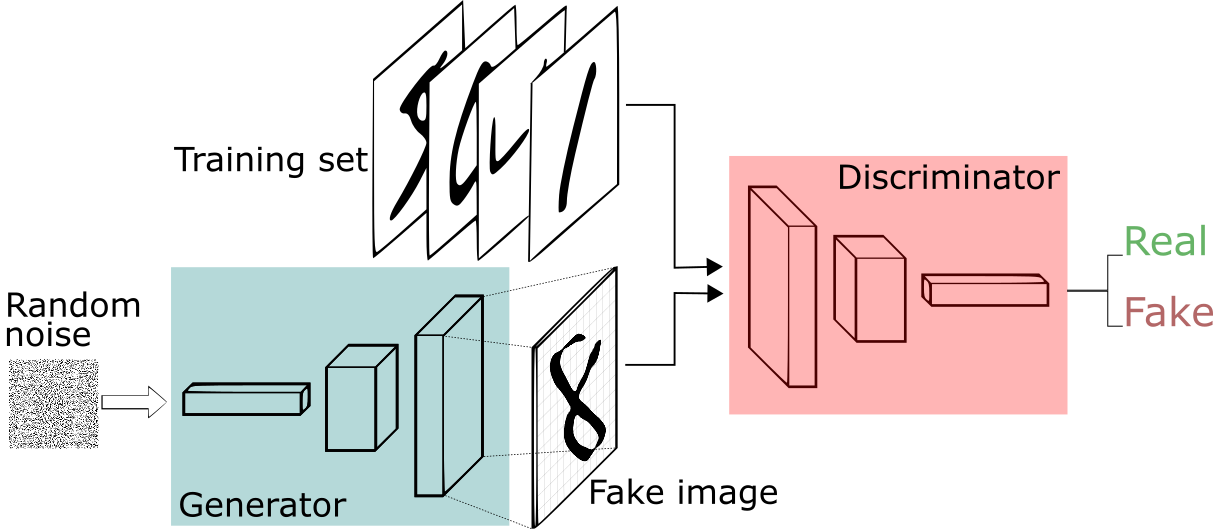
\includegraphics[width=\linewidth]{gan.png}
		\label{fig:gan}
	\end{figure}	
	
	\paragraph{}
	Este tipo de redes son bastante recientes, y están siendo ampliamente investigadas. Fruto de esas investigaciones, son nuevos tipos de GAN, como las DCGAN (\textit{Deep Convolutional Generative Adversial Network}), las cuales tratan de incorporar los métodos más recientemente creados para las redes convolucionales. 
	
	\paragraph{}
	También se encuentran las WGAN (\textit{Wasserstein Generative Adversial Network}), cuya principal motivación es analizar las distintas formas de medir la distancia entre la distribución del modelo \textit{p$_{G}$}, y la distribución real \textit{p$_{R}$}. Originalmente, las formulación de las GAN mostraba que la función objetivo para optimizar es la divergencia de \textit{Jensen-Shannon}. Sin embargo, para las WGAN, es utilizada la función de distancia \textit{Earth-Mover}, o distancia \textit{Wasserstein-1}, la cual intuitivamente calcula el coste del plan óptimo para transformar la distribución \textit{p$_{R}$} en \textit{p$_{G}$}. A continuación se especifica la fórmula:
	
	\begin{figure}[H]
	 	\centering
		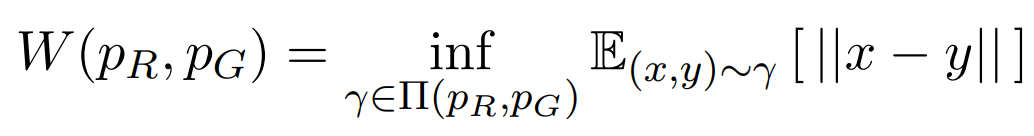
\includegraphics[height=1cm]{wasserstein.png}
		\label{fig:wasserstein}
	\end{figure}	
	
	\paragraph{}
	Dentro de las WGAN, también se pueden encontran las WGAN-GP (\textit{Wasserstein Generative Adversial Networks with Gradient Penalty}), las cuales surgieron como respuesta a que algunas configuraciones de las WGAN guiaban a muestras de baja calidad o completa falta de convergencia.
	
	\begin{figure}[H]
		\centering
		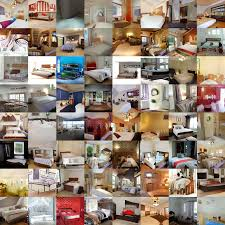
\includegraphics[width=6cm]{lsun.jpg}
		\label{fig:lsun_bedroom}
		\caption{Muestras creadas por una WGAN-GP entrenada en el conjunto de entrenamiento de habitaciones LSUN}
	\end{figure}	
	\newpage
	
	\section{Implementación}
	
	\newpage
	
	\section{Resultados}
	
	\newpage
	
	\section{Conclusiones}
	
	\newpage
	
	\begin{thebibliography}{9}
	\raggedright
	
	\bibitem{Fully convolutional network ensembles for white matter hyperintensities segmentation in MR images}
	H. Li, G. Jiang, J. Zhang, R. Wang, Z. Wang, W. Zheng y B. Menze. \textit{Fully convolutional network ensembles for white matter hyperintensities segmentation in MR images}, 2018
	
	\bibitem{Data Augmentation in Deep Learning}
	T. Neff. \textit{Data augmentation in deep learning using generative adversial networks}, 2018

	\end{thebibliography}
	
\end{document}